\chapter{Theory}
The main measurement principle by a \gls{gmr}-Sensor has been already described and characterized exhaustively by \citet{lit:thes:helou}, \citet{lit:thes:reisbeck} and \citet{lit:thes:brenner}. Therefore, this theoretical part will focus on (bio-)physical aspects of a cell rolling motion inside a microfluidic channel and surface modification chemistry.

\section{Microfluidics}

en Standardumfang wählen, Re, Navier Stokes, Scherraten, nicht newtonsche / newtonsche Fluide)
\subsection{Approximating the Navier-Stokes-Equation}

The main experiments of this work were carried out in microfluidic environments, which exhibit favorable properties compared to common turbulent systems. From a fluid-mechanical standpoint, shrinking the scales makes interfacial as well as electrokinetic phenomena much more significant, and reduces the importance of pressure and gravity.\cite{lit:fluidic:kirby} However, electodynamics, chemistry and fluid dynamics are incetricably intertwined, so that fluid flow can create electric fields (and vice versa), with a degree of coupling driven by the surface chemistry. Many of the resulting phenomena arise or can explained by Cauchy-Momentum equation (eq. \ref{eq:cauchymomentum}) and the resulting Navier-Stokes equation for incompressible fluids (eq. \ref{eq:navierstokes}).

\begin{align}
	\frac{\partial}{\partial t} \iiint \rho \mathrm{dV} &= - \iint \rho \mathbf{u} \cdot \vv{\mathbf{n}} \mathrm{dA} \\
	\nabla \cdot \mathbf{u} &= 0 \\
		\rho \frac{\partial \mathbf{u}}{\partial t} + \rho\mathbf{u} \cdot \nabla \mathbf{u} &= \nabla \cdot \boldsymbol{\tau} + \sum_{i}\mathbf{f}_i \label{eq:cauchymomentum} \\	
	\aunderbrace{\vphantom{\sum_{i}} \rho \frac{\partial \mathbf{u}}{\partial t}}_{\mathrm{Transient}} + \aunderbrace{\vphantom{\sum_{i}}\rho\mathbf{u} \cdot \nabla \mathbf{u}}_{\mathrm{Convection}} &= \aunderbrace{\vphantom{\sum_{i}}-\nabla p}_{\mathrm{Pressure}} + \aunderbrace{\vphantom{\sum_{i}}\eta \nabla^2 \mathbf{u}}_{\mathrm{Viscous}} + \aunderbrace{\sum_{i}\mathbf{f}_i}_{\mathrm{Body \ Forces}} \label{eq:navierstokes}
\end{align}
conservation of mass, momentum
reynolds number
\subsection{Flow and Shear in Microchannels with fiscous Vluids}
The foremost characteristic of a microchannel is the laminar flow behavior, which causes deterministic pathlines. Mathematically, this is described by the reynolds number, which compares the intertia to shear forces. If it results below a certain threshold of 2000, laminar flow can be assumed. This holds true for the utilized microfluidic with the dimensions \SI{12000}{\micro\meter} x \SI{700}{\micro\meter} x \SI{150}{\micro\meter} (l x w x h) and aequous buffer solutions, where the channel width was used as characteristic length $l$. Hence, simplifications of the Navier-Stokes equation can be applied to our system. 
\begin{equation}
	\mathit{Re}\ =\ \frac{2 \rho |\overline{u}| l }{\eta}
\end{equation}
The step from the Cauchy momentum equation to the Navier-Stokes equation is complex and harbors several sources of error. First, an incompressible newtonian fluid as well as channel is assumed. The used water suspensions can be approximated with negligible compressibility, which is not true for the real case. Also, for blood or other shear-thinning fluids some deviations are prone for high errors. This happens due to the fact that the \gls{tau} is decomposed into pressure and viscous contributions as shown in the equations \ref{eq:surfaceStressTensor}. Then, the divergence relation  of the respective viscous stress (eq. \ref{eq:divergence_Stresstensor}) does not hold for non-uniform viscosity $\eta$.
\begin{align}
	\boldsymbol{\tau} &= \boldsymbol{\tau}_{viscous} +  \boldsymbol{\tau}_{pressure} = 2\eta\epsilon - p \mathbf{I}_{\scaleto{3 \times 3}{4pt}} \label{eq:surfaceStressTensor}\\
	\nabla \cdot \boldsymbol{\tau}_{viscous} &= \nabla \cdot 2\eta\epsilon = \nabla \cdot \eta \nabla \mathbf{u} \ \underset{uniform}{\overset{only \ if \ \eta}{=}} \ \eta \nabla^2 \mathbf{u} 	\label{eq:divergence_Stresstensor}
\end{align}
Second, the channel height varies in reality as a result of fabrication inaccuracies. In the model case of a flow through a rectangular channel, no analytical solution of the Navier-Stokes equation exists, but a Fourier Series expansion if channel width is larger than channel height. \cite{lit:fluidic:bruus} The equation \ref{eq:flowVelocityRect} shows that height deviations can have prominent influence on a channel velocity simulation as it is proportional to $h^2$. Further, the flow rate (which is the velocity integral over the channel cross section) depends even on $h^3$. 
\begin{align}
 u   _x(y,z) = \frac{4 h^2 \Delta p}{\pi^3 \eta l} \sum_{n,odd}^{\infty} \frac{1}{n^3} \left( 1- \frac{\cosh (n \pi \frac{y}{h})}{\cosh (n \pi \frac{w}{2h})} \right) \sin (n \pi \frac{z}{h}) \label{eq:flowVelocityRect}
\end{align}
Third, the transient term (eq. \ref{eq:navierstokes}) was neglected in all simulations, but a connected syringe pump possesses a slow rise time (Fig. \ref{fig:fluidic:pumpStability:transient}) and a remaining ``pulsation error'' in steady state (Fig. \ref{fig:fluidic:pumpStability:steadystate}). In effect, another error adds to the simulation, which is only valid after several ten seconds of the last flow rate change.

\begin{figure}
	\begin{subfigure}[b]{0.5\textwidth}
		\centering
	    \addtocounter{subfigure}{1}  
		\subfigimg[clip,trim=115 100 80 60, height=100pt]{a} {./Ressources/Fluidic/Transient_SyringePump.jpg}		
		\addtocounter{subfigure}{-1}  
		\phantomsubcaption
		\label{fig:fluidic:pumpStability:transient}
	\end{subfigure}%
	\begin{subfigure}[b]{0.5\textwidth}
		\centering
		\addtocounter{subfigure}{1}  
		\subfigimg[height=100pt]{\textbf{b}}{./Ressources/Fluidic/SyringeSteadyState.eps}
		\addtocounter{subfigure}{-1}  
		\phantomsubcaption
		\label{fig:fluidic:pumpStability:steadystate}
	\end{subfigure}
\capption{Syringe Pump error sources}{Set flow rate: \orangeMLline, Real Flow Rate: \blueMLline \subref{fig:fluidic:pumpStability:transient} Transient step answer of a syringe pump through a microtube with \SI{254}{\micro\meter} inner diameter. \subref{fig:fluidic:pumpStability:steadystate} Steady state flow rate error around the desired \SI{5}{\micro\liter\per\minute} dispensing rate. A sinusoidal behaviour caused by the microstepping can be observed. \cite{lit:fluidic:fluigentPumpStability}}
\label{fig:fluidic:pumpStability}
\end{figure}

For later studies in a matlab model, the flow velocity and shear stress computations were carried out with the error sources considered. 



\subsection{Force Equilibrium of Microbeads}
Stokes Drag Force with lift correction
Gravity
Electro-static interaction
Magnetic Force
Friction
Interface-Forces
Faraus linquist
Protein interaction/ Avidity,Affinity
\subsubsection{Rolling Motion of Beads}
\clearpage
\subsection{}
\clearpage
\section{Surface Chemistry}
Introducing biological samples, such as peripheral whole blood and -plasma, into microsystems needs careful consideration of surface modification compared to buffered samples of adjusted pH containing cells or polymeric beads. Blood-material contact most often initiates surface-mediated reactions that lead to cell activation, blood clotting or biofilm formation.\todo{sources} In order to minimize unspecific interactions on surfaces, most contact faces are passivized with chemically and biologically inert materials or even composed entirely from it. In any use case, where a surface has to be functionalized with biomolecules, the intrinsic inertness then requires specialized methods for permanent and reproducible adhesion.\cite{lit:chem:surface:methods}

Molecules can be immobilized through various mechanisms on surfaces to achieve a biological or chemical functionality. The most simple is physisorption. Here, a biomolecule is bonded only by weak elektrostatic, van-der-Waals or dipole-dipole interaction with a adsorption enthalpy below \SI{50}{\kilo\joule\per\mole}.\todo{source} In contrast, this yields fast reaction rates, because no activation energy has to be overcome. Although a large number of molecules can be captured with this method, several drawbacks have been identified. \cite{lit:bio:ImmobilizationTechniques, lit:bio:immobilization:UV-ABs}
For example, immobilized receptors can desorb or move inside the channel, which in turn reduces sensitivity or causes false-positive results.\todo{Sensitivity und False-Positive Results sollten hier kurz dargestellt werden, zumindest in der Anwendung. } \cite{lit:bio:physisorp:desorption, lit:chem:surfModOptics} \\
Therfore, most functionalization approaches rely on chemisorption where molecules are covalently bound to a surface. Due to the higher activation energy barrier this bonding mechanism works slower in comparison to physisorption, though higher temperatures or catalysators can promote an equilibrium. One of the most well-known strategies to bring reproducible thin films on surfaces is the formation of \glspl{sam} where a dense layer of single molecules with high internal order forms upon dipping into a surface-active substance. \cite{lit:chem:sin:langeDiss}

\subsection{Surface Oxidation Methods}
Modifying a surface with functional silanes, requires oxidized sites, for example \gls{hydroxyl} resp. \gls{silanol} groups. In order to increase the presence of those reactive groups on substrates, various activation methods such as piranha, a mixture from \gls{h2o2} and \gls{h2so4}, \gls{o2} - plasma treatment or an \gls{hf} dip can be chosen. \cite{lit:chem:sin:etchingandchemical} 

Critical for any surface engineering is the internal structure and in consequence the binding energies of the surficial groups. The three mainly used substrates in this work, glass, \gls{pdms} and \gls{sin}, contain highly conserved, homogeneous surfaces and are mostly well characterized. The surface of glass exhibits already \gls{silanol} groups intrinsically and consequentially demands only a removal of impurities. \gls{pdms} and \gls{sin} however have different compositions as shown in Fig. \ref{fig:chem:func:substrate} and \ref{fig:chem:func:sin} hence requiring a strong oxidation agents to completely exchange its interface.  \cite{lit:chem:binding:sin, lit:chem:binding:pdms, lit:chem:surface:pdms}


\begin{figure}[h!]
	\begin{subfigure}[b]{0.30\textwidth}
		\centering
		\addtocounter{subfigure}{1}  
		\subfigimg[clip,trim=0 0 0 -40, width=\linewidth]{a} {./Ressources/Chemistry/Glass}		
		\addtocounter{subfigure}{-1}  
		\phantomsubcaption
		\label{fig:chem:func:glass}
	\end{subfigure}%
	\hfill
	\begin{subfigure}[b]{0.69\textwidth}
		\centering
		\addtocounter{subfigure}{1}  
		\subfigimg[clip, trim=0 0 575 120,width=\linewidth]{\textbf{b}}{Ressources/Chemistry/PDMS}
		\addtocounter{subfigure}{-1}  
		\phantomsubcaption
		\label{fig:chem:func:pdms}
	\end{subfigure}
	\capption{Different substrate surfaces: glass and \gls{pdms}}{Surface groups and internal structure of quartz glass (\textbf{a}) and \gls{pdms} (\textbf{b}). After an oxidation step, the methyl groups are changed to \gls{hydroxyl}.}
\end{figure}

\subsubsection{Piranha Solution}
Piranha is an oxidizer composed of \gls{h2o2} and \gls{h2so4}, typically in volume ratios between 1:3 and 1:7. The effectiveness of piranha in removing organic residues and creating \gls{hydroxyl} groups is induced by two distinct processes. In the first process, which is notably faster, hydrogen and oxygen are removed as units of water by the concentrated \gls{h2so4}.  (Reaction \ref{rct:pir1}) This occurs due to the thermodynamically very favorable reaction with an enthalpy of \SI{-880}{\kilo\joule\per\mole} and produces \gls{h2so5}, one of the strongest oxidants known.  \cite{lit:chem:piranha}

\begin{align}
	\ce{H2SO4 + H2O2 &-> H2SO5 + H2O} \label{rct:pir1}\\
	\ce{H2SO4 + H2O2 &-> HSO4- + H3O+ + O} \label{rct:pir2}
\end{align}

In another process the sulfuric acid boosts hydrogen peroxide from a mild oxidizer into the more aggressive atomic oxygen by the dehydration of \gls{h2o2}. (Reaction \ref{rct:pir2})  These two dehydration processes in the mixture result on the one hand in a highly corrosive nature against organic materials, particularly against the difficult to remove carbon. On the other hand, it is strongly acidic and oxidizing which in turn requires great care and substantial safety measures to prepare and use it harmlessly.\clearpage

\subsubsection{Hydrofluoric Acid}
\begin{wrapfigure}[7]{r}{.5\linewidth}
	\vspace{-1.35\baselineskip}
	\centering
	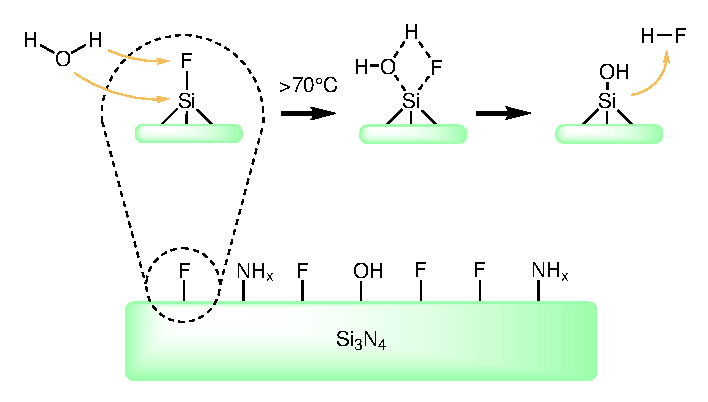
\includegraphics[width=1\linewidth]{Ressources/Chemistry/SiN}
	\capption{Proposed modification of \gls{sin} with \gls{hf}}{}
	\label{fig:chem:func:sin}
\end{wrapfigure}
One of the used substrates in this work is \gls{sin} as passivation layer above magnetic sensors as it has a significant better diffusion barrier against water or sodium ions and is chemically very inert. \cite{lit:chem:sin:surface} However, due to its complex crystal structure it is also difficult to modify by common chemicals and the exact surface composition still subject to scientific discussion. \cite{lit:chem:sin:etchingcontrol} Apart from cleaning the surface with piranha, few other modification methods have been reported, but only one suitable for the direct generation of \gls{hydroxyl} groups.

There, as depicted in \ref{fig:chem:func:sin}, the reaction \ch{Si-OH + HF <-> Si-F + H2O} takes place reversibly due to the coincidence that \ch{Si-O} and \ch{O-H} as well as \ch{Si-F} and \ch{H-F} bonds have similar binding energies and hence the forward and reverse reactions a low activation energy. After Le Chatelier's principle, a depletion of \gls{hf} in the bulk leads then to an increase in surficial hydroxyl groups. \cite{lit:chem:sin:SiFSiOH} In further works, it has been determined that an oxidation with a similar protocol based on aequous \gls{hf} yields a variable \gls{siloxane} coverage with \SI{37(17)}{\percent} of a monolayer, which nevertheless can be used for stable, covalent attachment of silanes.  Nominally the same surface coverages of silicon oxide and nitride surfaces could be achieved by ethoxy- and chlorosilanization. \cite{lit:chem:sin:surfacEtchingandMod} As shown by \citep{lit:chem:sin:silane}, the subsequent surfaces exhibit beneficial biological properties and can be modified by further standard procedures.


\subsubsection{Oxygen Plasma}
Apart from wet chemistry methods, the exposure of a surface to oxygen plasma yields \gls{hydroxyl} groups as well. In a plasma chamber, a low-pressure gas is irradiated by \si{\kilo\hertz} to \si{\mega\hertz} waves to excite and ionize its atoms. In consequence, the UV-radiation emitted by the gas can photolyse typical organic bonds and remove surface contaminations. Additionally, reactive oxygen species such as \ce{O2+}, \ce{O2-}, \ce{O3} or \ce{O} either oxidize the surface as well or bind dissociated components with low vapor pressure. During an evacuation in the process, these molecules are removed from the chamber intrinsically. \cite{lit:chem:plasma}  

\subsection{Silane Chemistry}

By the use of silane chemistry a surface is rendered organofunctional with alkoxysilane molecules. Since glass, silicon, alumina, titania, and quartz surfaces, as well as other metal oxide interfaces, are rich in hydroxyl groups, silanes are particularly useful for modifying these materials. \cite{lit:chem:silanizingGlass}\\The general formula for a silane coupling agent (Fig. \ref{fig:chem:trialkoxysilane}) typically shows the two classes of functionality. X is a hydrolyzable group typically alkoxy, acyloxy, halogen or amine.
\\\begin{wrapfigure}[9]{r}{.25\linewidth}
	\vspace{-0.7\baselineskip}
	\centering
	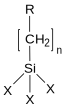
\includegraphics{Ressources/Chemistry/Trialkoxysilan}
	\capption{Trialkoxysilane}{Structure of a typical trialkoxysilane, X: hydrolyzable group, R: non-hydrolyzable organic radical, n: methylene chain-length}
	\label{fig:chem:trialkoxysilane}
\end{wrapfigure} 
Following hydrolysis, a reactive \gls{silanol} group is formed, which can condense with other silanol groups to form \gls{siloxane} linkages. 
(Fig. \ref{fig:chem:APTES}) Stable condensation products are also formed with other oxides such as those of aluminum, zirconium, tin, titanium, and nickel. Less stable bonds are formed with oxides of boron, iron, and carbon, whereas alkali metal oxides and carbonates do not form stable bonds with \glspl{siloxane} at all. The R group (Fig. \ref{fig:chem:trialkoxysilane}) is a nonhydrolyzable organic radical that may posses a functionality that imparts desired characteristics. One of the more common silanes is \gls{aptes}, where the X group consists of an \gls{ethoxy} group, the organic rest R is substituted by an \gls{amine} and the 3 \gls{methylene} groups alter \textit{n} to 3. \cite{lit:chem:GELEST} 
\begin{figure}[h]
	\centering
	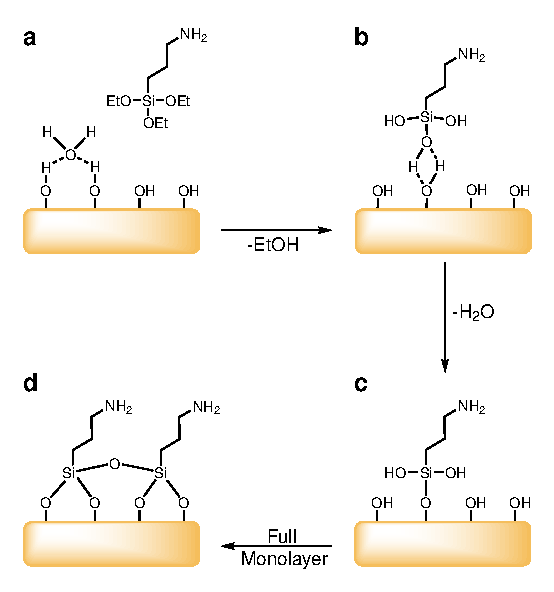
\includegraphics[width=1\linewidth]{./Ressources/Chemistry/APTES.eps}
	\capption{APTES Modifcation of an oxidized surface}{\textbf{a} Before the condensation reaction, the oxidized surface forms hydrogen bonds with water molecules. The silane molecules are in the bulk solution. \textbf{b} The hydrolyzed \gls{silanol} group adsorbs onto the surface and forms hydrogen bridges with it. \textbf{c} In a condensation reaction, under the loss of water, a covalent bond to the surface forms. \textbf{d} After the \gls{sam} assembly the surface is saturated with a covalent-bound, crosslinked silane film. \cite{lit:chem:aptes:SilaneReaction}}
	\label{fig:chem:APTES}
\end{figure}

The final result of reacting an organosilane with a substrate ranges from altering the wetting or adhesion characteristics of the substrate, utilizing the substrate to catalyze chemical transformation at the heterogeneous interface, ordering the interfacial region, and modifying its partition characteristics. Significantly, it includes the ability to effect a covalent bond between organic and inorganic materials. Especially in optical or biological sensors, silane modifications open a broad range of applications. 

However, the silanization reactions bear a few drawbacks which are often neglected. For instance, silane chemistry is strongly temperature and pH-dependent. \cite{lit:chem:silaizationTemp,lit:chem:silanizationParameters} Further, in a process to build \glspl{sam} out of \gls{aptes}, the reaction has to be catalyzed by water. But already small changes in the water content cause dramatic deviations in layer thickness. \cite{lit:chem:sin:selectivemod} Additionally, silanes can crosslink to themselves through possible side reactions. (Fig. \ref{fig:chem:APTES} D) \cite{lit:chem:aptes:Crosslink}



\subsection{Carbodiimide Crosslinker Chemistry}
The in previous manner produced \gls{amine}-terminated films by \gls{aptes} form the basis of many reactions and open the possibility to various applications, such as the direct attachment of biofunctional molecules by carbodiimide crosslinking chemistry.\cite{lit:bio:BioconjugateTechniques} Here, \gls{carboxyl} groups are modified by \gls{edc} and \gls{nhs} to form a stable secondary \gls{amide} bond with any primary \gls{amine}.

\begin{figure}[htb!]
	\centering
	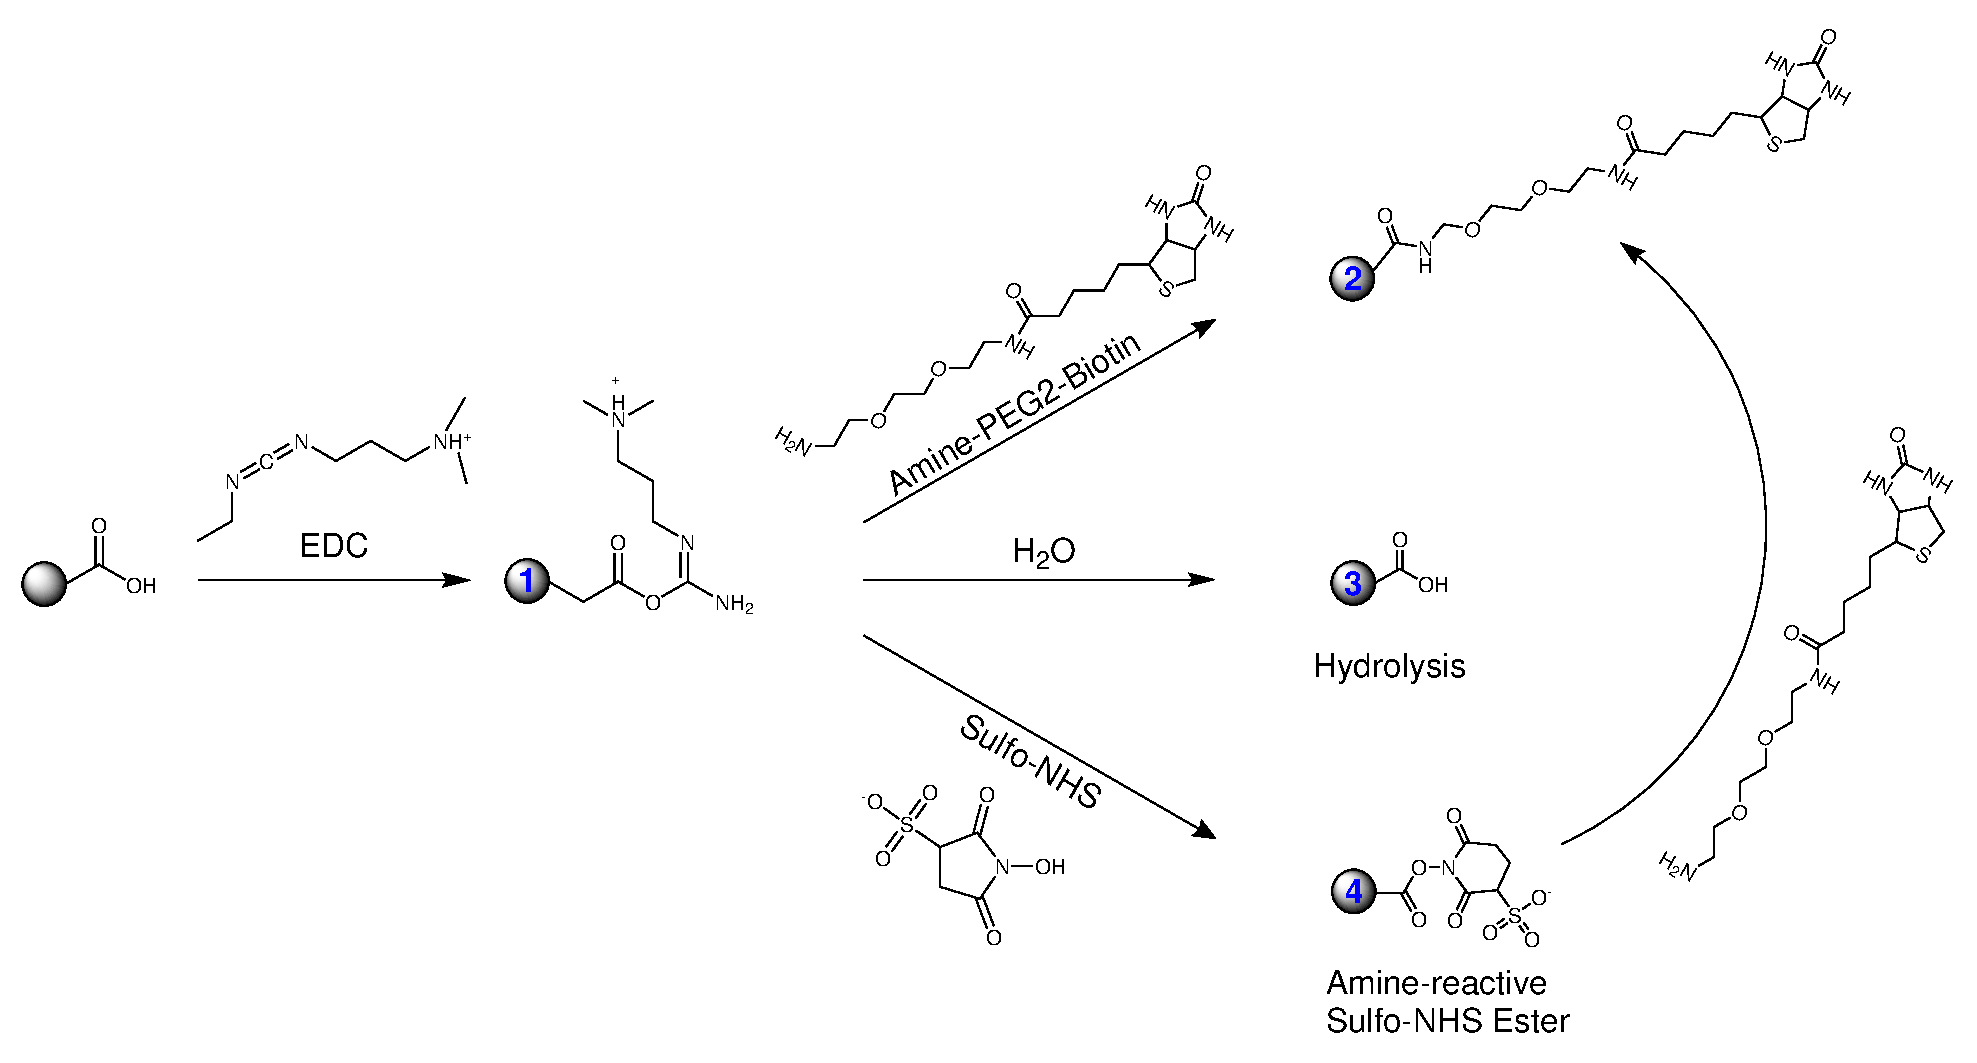
\includegraphics[width=\linewidth]{./Ressources/Chemistry/EDC-NHS.eps}
	\capption{Carboxyl bead modification with EDC/NHS}{The carboxy groups bead are activated with \gls{edc} to an active O-acylisourea intermediate. This can then either be nucleophilicly attacked by a primary amine of the amine-PEG$_2$-biotin reactant or - due to its instability - hydrolzed back to a regenerated carboxyl surface. A present NHS-ester can also displace the O-acylisourea to form a considerably more stable intermediate which then itself reacts with any primary amine.}
	\label{fig:chem:COOH-EDC-NHS}
\end{figure}
\clearpage
The general reaction mechanism is depicted in Fig. \ref{fig:chem:COOH-EDC-NHS} for the example of a microbead surface, but it can equivalently be applied to any other modified surface or molecule. The initial \gls{carboxyl} group is esterified by \gls{edc} to an active o-acylisourea intermediate and leaves rapidly upon nucleophilic attack of an amine with release of an iso-urea byproduct. A zero-length amide linkage is formed. (Fig. \ref{fig:chem:COOH-EDC-NHS}, 1->4) Sulfhydryl and hydroxyl groups also will react with such active esters, but the products of such reactions, thioesters and esters, are relatively unstable compared to an \gls{amide} bond. (Fig. \ref{fig:chem:COOH-EDC-NHS}, 1)\newline
However, this reactive complex is slow to react with amines and can hydrolyze in aqueous solutions, having a rate constant measured in seconds. If the target amine does not find the active \gls{carboxyl} before it hydrolyzes (Fig. \ref{fig:chem:COOH-EDC-NHS}, 3), the desired coupling cannot occur. This is especially a problem when the target molecule is in low concentration compared to water, as in the case of protein molecules. Notwithstanding, forming a \gls{nhs} ester intermediate from the reaction of the \gls{hydroxyl} group on NHS with the \gls{edc} active-ester complex increases the resultant amide bond formation remarkably. (Fig. \ref{fig:chem:COOH-EDC-NHS}, 3->4) \cite{lit:chem:nhs2}

Another critical point in carbodiimide chemistry is the solubility of the compounds. \gls{edc}, \gls{nhs} and \gls{snhs} are soluble in aqueous and organic solvents. Nevertheless, activation  with  non-sulfonate \gls{nhs} decreases water-solubility of the modified carboxylate molecule, while activation with \gls{snhs} preserves or increases its water-solubility by virtue of the charged sulfonate group. \cite{lit:chem:snhs}

\clearpage

\subsection{Microscopic Particle Surface Physics}
\todo{write!!!!}


\subsection{The Biotin-Avidin-System}
Until now, the interaction of the homotetrameric protein avidin and its ligand biotin forms one of the strongest known non-covalent bonds in biological systems characterized by a \gls{kd} in the range of \SI{e-15}{\molar}.\cite{lit:bio:biotin:avidin_discovery} First isolated from chicken egg white, it became a standard to use in biotechnology when researchers found a similar bacteria protein - streptavidin - in \textit{Streptomyces} strains.\cite{lit:bio:biotin:discovery} However, the charged glycoprotein avidin exhibits unspecific binding in some assays in comparison to streptavidin. Therefor, several companies developed deglycosylated forms of avidin with a neutral isoelectric points to minimize unspecificity. (NeutrAvidin, Extravidin, NeutraLite) In recent studies, a mutant streptavidin called ``Traptavidin'' exhibitied an even 10 times dissociation rate.\cite{lit:bio:biotin:engStrep}
As discovered in the early 1990s, biotin is bound inside a highly stable $\beta$-barrel structure, and stabilized by hydrogen bonds and van der Waals forces.\cite{lit:bio:biotin:bindingmechanism} In a unique mechanism, a side group of biotin (valerate) binds to a neighboring monomer of streptavidin and therefor stabilizes the dimer complex intrinsically.\cite{lit:bio:biotin:binding,lit:bio:biotin:freeenenergy} From a thermodynamical point-of-view, the interaction of the vitamin and protein is described by a total free binding energy of \SIrange{300}{330}{\kilo\joule\per\mole} for a tetrameric protein. \cite{lit:bio:biotin:freeenenergy}  All these aspects lead to a significant rupture force for the biotin-release of \SI{250}{\pico\newton}.\cite{lit:bio:biotin:rupture}

\begin{figure}[tbph!]
		\begin{subfigure}[b]{0.4\textwidth}
		\centering
		\addtocounter{subfigure}{1}  
		\subfigimg[height=150pt]{\textbf{a}}{./Ressources/Biology/biotin.eps}
		\addtocounter{subfigure}{-1}  
		\phantomsubcaption
		\label{fig:biotin}
	\end{subfigure}%
		\begin{subfigure}[b]{0.59\textwidth}
		\centering
		\addtocounter{subfigure}{1}  
		\subfigimg[clip, height=150pt]{b}{Ressources/Biology/crystalAvidin_bindingSite.png}		
		\addtocounter{subfigure}{-1}  
		\phantomsubcaption
		\label{fig:crystalavidin}
	\end{subfigure}%
	\capption{Functional Structures of Biotin and Streptavidin}{(\textbf{a}) Biotin chemical structure, (\textbf{b}) Homotetrameric Streptavidin with the anchor point at one terminus.\cite{lit:bio:SA:crystal}}
	\label{}
\end{figure}



\section{Magnetoresistive Sensing}
Short intro in GMR
Short intro over MRCyte


